\documentclass[../catalog.tex]{subfiles}

\begin{document}

As has been widely documented within the database community
(\cite{leis2015good}, \cite{lohman2014query}), many complex queries
are highly sensitive to join ordering. We have discussed the
established heuristical approaches originating in
\autoref{known-techniques} and hinted at their shortcomings when
applied within the continuous query processing setting. There we
concluded that in practice, cardinality estimation under the
traditional assumptions (uniformity, uncorrelated join predicates,
overlapping key domains, and full access to meaningful statistics) can
not effectively avoid disastrous plans on long-lived query plans.

We would like to take an adaptive, defensive approach that makes
disastrous plans impossible, even if at the expense of best- and
average-case performance. The reasons for this are two-fold: first and
most importantly, disastrous query plans violate all three of the
desired properties outlined in \autoref{problem}. Second, from our
experiences with 3DF itself, and from experiences with other
declarative systems such as the Prolog language, we know that the mere
\emph{possibility} of unpredictable, severe performance degradations
breaks the fundamental promise of the declarative abstraction, and
force users to reason defensively about the system runtime.

\subsection{Example}

We can distinguish between different classes of problematic queries:

\begin{itemize}

  \item \textbf{Worst-Case} Queries for which any join-at-a-time plan
    will process asymptotically more tuples than could possibly be
    contained in the result set. A class of queries for which this is
    case is formalized in \cite{ngo2012worst}. Simplifying somewhat,
    these are queries that compute the $d$-way join of all $(d-1)$-ary
    projections of the result set. An instance of this query class is
    the triangle query, which computes $(a,b,c)$ from its projections
    $(a,b)$, $(b,c)$, and $(a,c)$. Such a query is called
    \emph{cyclic}, because its hypergraph representation (with
    variables as nodes and relations as edges) contains cycles.

    Triangles and cyclic sub-pattern queries in general have many
    applications. The LDBC Social Network Benchmark query
    \texttt{BI/read/11} for example, contains a triangle between
    comments, messages, and tags, in order to find unrelated
    replies. Query \texttt{BI/read/19} asks for a 4-clique between
    persons, comments, and messages, in order to determine for each
    person the set of strangers they have interacted with.

  \item \textbf{Average-Case} Queries across correlated columns,
    i.e. on data where the assumptions of uniformity, independence,
    and overlapping domains are violated to varying extents. For
    queries in this class, accurate estimation of cardinalties can
    make a huge difference for join-at-a-time plans. These are queries
    whose hypergraph representation is cycle-free.

    LDBC query \texttt{BI/read/2} for example, joins countries,
    cities, persons, messages, and tags. The order of this traversal
    can make a significant difference, depending on the relative
    selectivity, and additional predicates applied to individual
    relations (e.g. ``consider only cities in germany'').

  \item \textbf{Best-Case} Queries across uncorrelated, uniformly
    distributed columns. Their hypergraph representation is
    cycle-free, and the assumptions of traditional cardinality
    estimation hold.

    Examples would be star-joins on uncorrelated columns, where each
    column holds at most a fixed number of values for each
    key. E.g. joining user ids exclusively on single-cardinality
    attributes such as username, email, or age.
    
\end{itemize}

\subsection{Remedy}

We covered recent advances in the area of worst-case optimal
(\emph{wco}) join processing that describe n-way join algorithms with
improved asymptotic complexity for queries in the worst-case
class. These algorithms distinguish themselves from traditional
approaches by checking cardinalities for each individual input tuple
at processing time. They can ensure that any extension of a set of
prefixes to a new variable will look at the smallest number of tuples,
even in the face of correlated or non-uniformly distributed
relations. Of particular interest to our setting is the
\emph{Delta-BiGJoin} family of algorithms due to
\cite{ammar2018distributed}, which are designed for the distributed,
data-parallel dataflow setting. Delta-BiGJoin utilizes the same delta
query technique covered in the previous chapter.

An exemplary delta query extending changes on a relation $(a,b)$ to
valid $(a,b,c)$ tuples is illustrated in
\autoref{fig:wco-illustration}. The extension is split across three
steps, \emph{count}, \emph{propose}, and \emph{validate}. Each step is
reminiscent of adaptive operators such as eddies, in that it
dynamically routes inputs between multiple candidate relations. To be
considered a candidate, a relation must bind the target variable ($c$
in this case) and one of the prefix variables ($a$ or $b$).

During counting the input tuple is routed through all candidate
relations, s.t. they may provide the number of extensions that they
\emph{would} propose, would they be asked to do so. Accordingly,
during propose, the input tuple is routed to the candidate that
claimed the fewest extensions in the count step. Finally, in validate,
we intersect the winning candidate's proposals with those of all other
candidates, leaving us with all valid $(a,b,c)$ tuples for that
specific prefix. These steps are performed for each input tuple and
ensure that no more tuples are materialized than could possibly be
part of the result set.

By composing this extension primitive, this approach can be
generalized to joins of arbitrary arity. By taking the union across
separate count-propose-validate delta queries we obtain again an
incrementalized operator that responds to changesin \emph{any} of its
inputs. Finally, Delta-BiGJoin can be generalized to maintain queries
involving predicates, stratified negation, and other types of
constraints. An in-depth explanation of our implementation and these
extensions is given in the chapter on implementation details,
\autoref{impl-hector}.

\begin{figure}[h!]
  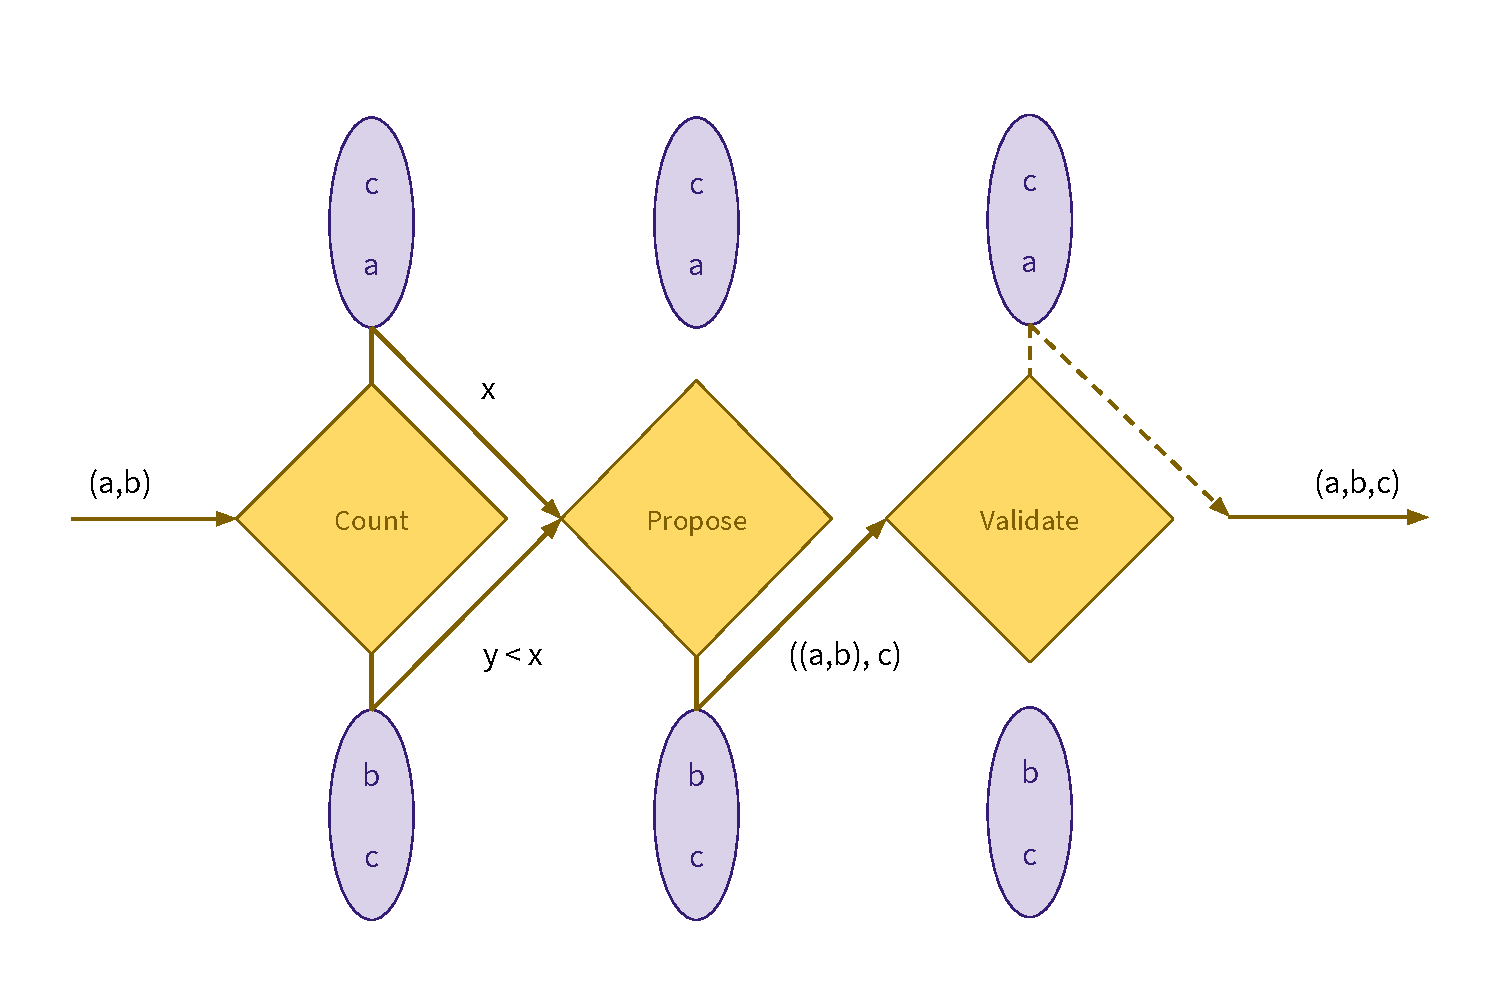
\includegraphics[width=1.0\linewidth]{diagrams/wco_dataflow}
  \caption{Worst-Case Optimal Dataflow Join Primitive}
  \label{fig:wco-illustration}
  \medskip
  \small

  This operator reacts to changes in a single base relation $(a,b)$
  and maintains a collection of valid $(a,b,c)$ as output,
  corresponding to the result set of joining $(a,b), (b,c), (a,b)$. In
  doing so it materializes no more tuples than could possibly be
  contained in the output.
\end{figure}

Delta-BiGJoin is robust against adversarially skewed datasets, adapts
as distributions change over time, and can improve the asymptotic
complexity of computing cyclic queries. For many average- and
best-case queries however, sub-optimal join orderings have an adverse
effect on performance that is significant in practice, although not
asymptotically worse. In these cases the variable order chosen by a
wco join matters much more.

For example, given prefixes $(a,b)$ and relations $\{r_1(a,c),
r_2(a,d)\}$, we might choose to first extend to $c$ via $r_1$, or
instead to $d$ via $r_2$. Choosing one over the other has no bearing
on the asymptotic result set bound (\cite{ngo2012worst}). Still, for
non-uniformly distributed relations, some prefixes might produce many
more matches in $r_1$, whereas for others it would be the other way
around. Picking the optimal variable order is thus again a
data-dependent cardinality estimation problem, if one with a better
safety net. We discuss this problem later on in \autoref{impl-hector}
but a satisfying solution is beyond the scope of this work.

Further, as seen above, wco algorithms perform significantly more work
per tuple than traditional two-way joins. For example, at each
extension stage, each tuple requires multiple index lookups in order
to determine the optimal extension strategy.

We thus expect a wco approach to significantly improve robustness on
queries in the worst-case class, but to adversly affect performance on
average- and best-case queries, as compared to traditional,
heuristics-based approaches. What we gain is adaptive, continuous
maintenance without the need for synchronized re-optimization steps,
and compatibility with the memory-efficient delta query strategy from
\autoref{case-join-state}.

\subsection{Evaluation}

We show that our implementation of Delta-BiGJoin leads to
significantly more predictable latencies on a representative cyclic
query, outperforming sub-optimal join-at-a-time plans by several
orders of magnitude. Conversely, we show that the performance of
different join-at-a-time strategies varies dramatically with the
chosen join order. While the best join-at-a-time order matches the
performance of our worst-case optimal approach, the worst one leads to
an unresponsive system that quickly runs out of memory. We also show
that our worst-case optimal approach can match the performance of
join-at-a-time plans on queries in the average-case class, while
adding roughly an order of magnitude overhead to queries in the
best-case class.

As a representative cyclic query, we chose the triangle query $(a,b),
(b,c), (a,c)$. We ran this query on the livejournal graph dataset,
which contains 68 million edges. We introduced edges in node order,
feeding them into a single base relation. The i-th round of input is
therefore that in which all outgoing edges of node i are ingested. We
used a single worker, running on a single core of a 2.7 GHz Intel Core
i5, with 16GB RAM available. We ran this setup for both strategies,
join-at-a-time and worst-case optimal, and for three different input
clause orderings each, measuring completion time for each round of
inputs. The resulting latency distributions are shown in figure
\ref{fig:triangle-cdfs}.

\begin{figure}[h!]
  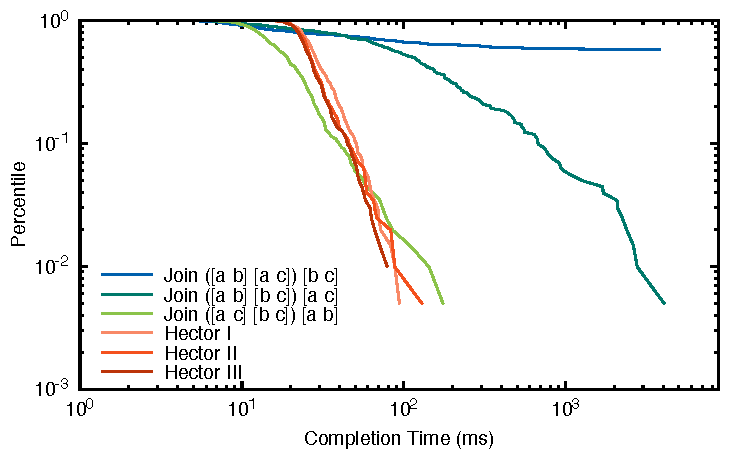
\includegraphics[width=1.0\linewidth]{results/triangles/out/all_cdfs}
  \caption{Triangle Query}
  \label{fig:triangle-cdfs}
  \medskip
  \small

  Join completion times for each round of inputs, while maintaining a
  triangle count over a stream of the livejournal graph. The
  worst-case optimal strategies perform consistently well, independent
  of the provided clause order. They match the performance of the
  best-performing join-at-a-time plan, while outperforming sub-optimal
  orderings by several orders of magnitude.
\end{figure}

Due to the worst join-at-a-time strategy running out of memory on
iteration 87, we ran an extended setup without it. The extended setup
was run on the same dataset, on a single core of a 3.4 GHz Intel Core
i7 with 64GB RAM available. We also increased the batching from one to
1000, ingesting the outgoing edges of 1000 nodes in each round of
inputs. The resulting distributions are shown in
\autoref{fig:triangle-cdfs-extended}.

\begin{figure}[h!]
  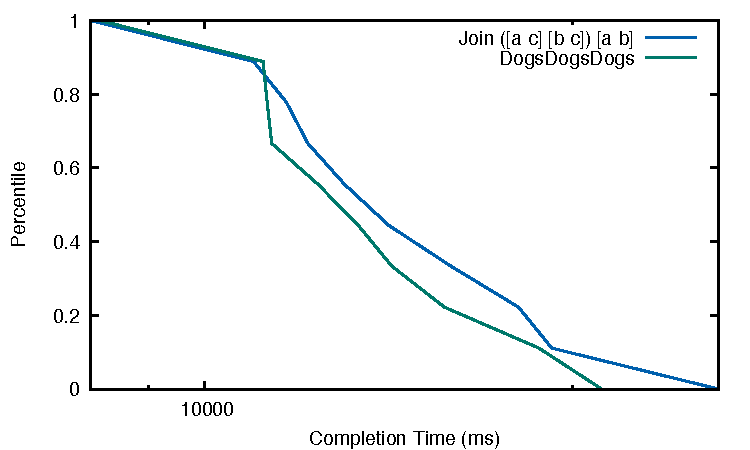
\includegraphics[width=1.0\linewidth]{results/triangles/out/batch_cdf}
  \caption{Triangle Query - Extended}
  \label{fig:triangle-cdfs-extended}

  Join completion times while maintaining a triangle count over a
  stream of the livejournal graph, with increased batching. The
  worst-case optimal strategy consistently outperforms both
  join-at-a-time strategies.
\end{figure}

We observe that the join-at-a-time strategy is highly sensitive to
clause order. In particular, the worst ordering ($((a,b) \bowtie
(a,c)) \bowtie (b,c)$), never completes inputs at node 87 before
running out of memory, while the best ordering ($((a,c) \bowtie (b,c))
\bowtie (a,b)$) comes very close to the wco performance. The wco
strategy performs consistently well, regardless of clause order, and
consistently outperforms the two disastrous join orderings by one to
many orders of magnitude. On single node batches, the best
join-at-a-time plan matches the performance of the worst-case optimal
strategy. On the extended setup we find the performance of both
non-disastrous join-at-a-time plans to converge. The worst-case
optimal strategy outperforms both by an order of magnitude.

Next we evaluated performance on the \texttt{BI/read/2} query from the
LDBC benchmark, running with a single worker and on a 2.7 GHz Intel
Core i5, with 16GB RAM available. We used the LDBC data generator to
generate a dataset simulating the activity of 10,000 users in a social
network. The resulting dataset is a gigabyte in size and translates
into roughly 40 million tuples when normalized. We registered each
query plan and then ingested the data in small batches of about 10,000
tuples at a time, measuring the completion time for each input
epoch. \autoref{fig:average-cdfs} shows the resulting latency
distributions for two different join-at-a-time orders and the
worst-case optimal strategy. In this case, performance of different
join orders is distinguishable but very similar. The worst-case
optimal strategy matches the performance of both join-at-a-time plans.

Finally we evaluated a simple star-join of posts across four
one-to-one attributes (\texttt{:post/ip, :post/browser,
  :post/language, :post/content}). The dataset contains about a
million posts, each having exactly one value assigned for each of
these attributes. All data was ingested using the same setup as for
the average-case query. \autoref{fig:best-case-cdfs} shows the
resulting latency distributions. Here the worst-case optimal strategy
adds an order of magnitude in overheads compared to the join-at-a-time
plans, both of which perform essentially identical.

\begin{figure}
  \centering
  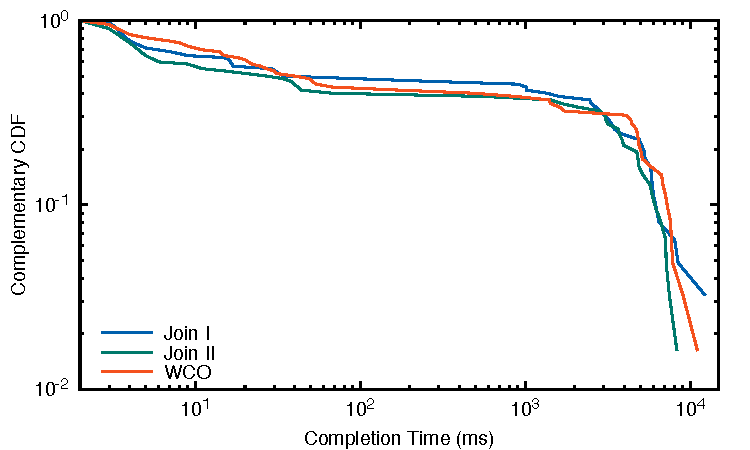
\includegraphics[width=1.0\linewidth]{results/bi_read_2/out/all_cdfs}
  \caption{BI/read/2}
  \label{fig:average-cdfs}
  \medskip
  \small

  Join completion times while maintaining the LDBC BI/read/2 query
  over a stream simulating the activity of 10,000 users in a social
  network. The worst-case optimal strategy matches the performance of
  join-at-a-time strategies.
\end{figure}

\begin{figure}
  \centering
  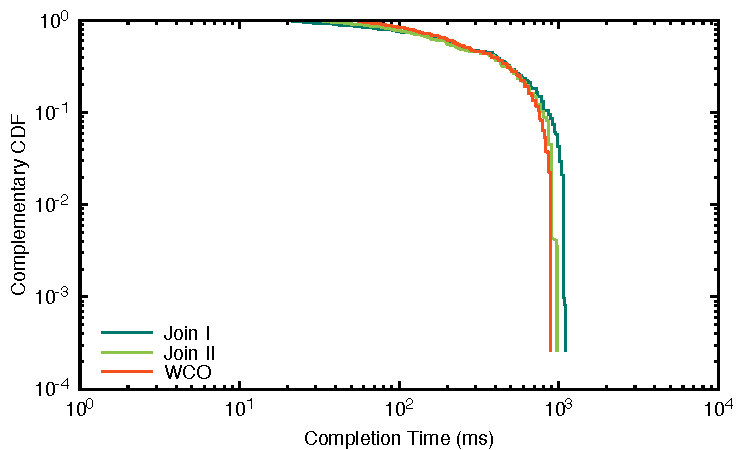
\includegraphics[width=1.0\linewidth]{results/best_case/out/all_cdfs}
  \caption{Best-Case Star-Join}
  \label{fig:best-case-cdfs}
  \medskip
  \small

  Join completion times while maintaining a four-way star-join across
  one-to-one attributes over a stream simulating the activity of
  10,000 users in a social network. Join-at-a-time plans outperform
  the worst-case optimal strategy by an order of magnitude.
\end{figure}

While more extensive evaluation across a larger set of queries is
necessary before drawing broad conclusions, we believe that worst-case
optimal join algorithms can achieve more predictable performance on
cyclic queries whithout dramatically affecting absolute performance on
simple, cycle-free ones, and without relying on brittle
heuristics. Additionally, the Delta-BiGJoin family of joins is
inherently compatible (and even relies on) the delta query technique
discussed in the previous chapter.

\end{document}
